\documentclass[a4paper,11pt,oneside]{article}

% To use this template, you have to have a halfway complete LaTeX
% installation and you have to run pdflatex, followed by bibtex,
% following by a one-two more pdflatex runs.
%
% Note thad usimg a spel chequer (e.g. ispell, aspell) is generolz
% a very guud ideo.

\usepackage[utf8]{inputenc}
\usepackage[a4paper,top=3cm,bottom=3cm,left=3cm,right=3cm]{geometry}
\renewcommand{\familydefault}{\sfdefault}
\usepackage{helvet}
\usepackage{csquotes}
\usepackage[english]{babel}     %% typographie française
\usepackage[style=numeric,language=english]{biblatex}
\usepackage{parskip}        %% blank lines between paragraphs, no indent
\usepackage[margin=1cm]{caption}%% give long captions a margin
\usepackage{booktabs}           %% typesetting nice tables
\usepackage[pdftex]{graphicx}    %% include graphics, preferrably pdf
\usepackage[pdftex]{hyperref}
\usepackage[T1]{fontenc}    %% many PDF options can be set here
\pdfadjustspacing=1        %% force LaTeX-like character spacing

\newcommand{\myname}{Joe Sample}
\newcommand{\mytitle}{On the Possibility of the Impossible}
\newcommand{\mysupervisor}{Prof.~V.~Confused}

\hypersetup{
    pdfauthor = {\myname},
    pdftitle = {\mytitle},
    pdfkeywords = {},
    colorlinks = {true},
    linkcolor = {blue}
}

\addbibresource{bsc-sample.bib}

\begin{document}
    \pagenumbering{roman}

    \thispagestyle{empty}

    \begin{flushright}
        
\includegraphics[scale=0.8]{bsc-logo}
    \end{flushright}
    \vspace*{40mm}
    \begin{center}
        \huge
        \textbf{\mytitle}
    \end{center}
    \vspace*{4mm}
    \begin{center}
        \Large by
    \end{center}
    \vspace*{4mm}
    \begin{center}
        \LARGE
        \textbf{\myname}
    \end{center}
    \vspace*{20mm}
    \begin{center}
        \Large
        Bachelor Thesis in Computer Science
    \end{center}
    \vfill
    \begin{flushleft}
        \large
        Submission: \today \hfill Supervisor: \mysupervisor \\
        \rule{\textwidth}{1pt}
    \end{flushleft}
    \begin{center}
        Jacobs University Bremen $|$ Department of Computer Science and Electrical Engineering
    \end{center}

    \newpage
    \thispagestyle{empty}

    \subsection*{English: Declaration of Authorship}

    I hereby declare that the thesis submitted was created and written
    solely by myself without any external support. Any sources, direct
    or indirect, are marked as such. I am aware of the fact that the
    contents of the thesis in digital form may be revised with regard to
    usage of unauthorized aid as well as whether the whole or parts of
    it may be identified as plagiarism. I do agree my work to be entered
    into a database for it to be compared with existing sources, where
    it will remain in order to enable further comparisons with future
    theses. This does not grant any rights of reproduction and usage,
    however.

    This document was neither presented to any other examination board
    nor has it been published.

    \subsection*{German: Erklärung der Autorenschaft (Urheberschaft)}

    Ich erkläre hiermit, dass die vorliegende Arbeit ohne fremde Hilfe
    ausschließlich von mir erstellt und geschrieben worden ist. Jedwede
    verwendeten Quellen, direkter oder indirekter Art, sind als solche
    kenntlich gemacht worden. Mir ist die Tatsache bewusst, dass der
    Inhalt der Thesis in digitaler Form geprüft werden kann im Hinblick
    darauf, ob es sich ganz oder in Teilen um ein Plagiat handelt. Ich
    bin damit einverstanden, dass meine Arbeit in einer Datenbank
    eingegeben werden kann, um mit bereits bestehenden Quellen
    verglichen zu werden und dort auch verbleibt, um mit zukünftigen
    Arbeiten verglichen werden zu können. Dies berechtigt jedoch nicht
    zur Verwendung oder Vervielfältigung.

    Diese Arbeit wurde noch keiner anderen Prüfungsbehörde vorgelegt
    noch wurde sie bisher veröffentlicht.

    \vspace{20mm}

    Date, Signature

    \newpage

    \section*{Abstract}

    % TODO: add this reference
    % http://www.cs.unc.edu/~fuchs/publications/VisSurfaceGeneration80.pdf


    Constructive Solid Geometry (CSG) is a method used in computer graphics, computer aided design, generic modelling languages, and many more applications to construct complex geometries from simple primitives or polyhedral solids by using boolean operators, namely union, difference, and intersection. The method becomes especially interesting when implemented in a ray tracing system as the core problem translates to executing arithmetic logic on a pair of uni-dimensional rays. However, most existing ray tracing systems generally suffer from the cost of the expensive object space intersection computation, and the generic CSG algorithms suffer immensly from their computational complexity, making it very difficult to integrate into working rendering engines.

    (target size: 15-20 lines)

    \newpage
    \tableofcontents

    \clearpage
    \pagenumbering{arabic}


    \section{Introduction}

    This, like the rest, addresses fellow experts from your field (but
    not from your particular topic of research). Here you should
    technically connect to the main concepts from that field and give an
    outline of your project, stating the research/engineering question
    that you want to get answered by your project.

    (target size: 1-2 pages)


    \section{Related Works}

    This part should make clear which question, exactly, you are
    pursuing, and why your project is relevant/interesting.
    This is the place to explain the background and to review the existing
    literature.
    Where does your project extend the state of the art?
    What weaknesses in known approaches do you hope to overcome? If you
    have carried out preliminary experiments, describe them here.

    (target size: 5-10 pages)


    \section{Constructive Solid Geometry}

    This is the technical core of the thesis. Here you lay out your how
    you answered your research question, you specify your design of
    experiments or simulations, point out difficulties that you
    encountered, etc.

    (target size: 5-10 pages)


    \section{Optimization}

    This section discusses criteria that are used to evaluate the
    research results. Make sure your results can be used to published
    research results, i.e., to the already known state-of-the-art.

    (target size: 5-10 pages)

    \begin{table}[ht]
        \begin{center}
            \begin{tabular}{cl}
                \toprule
                Number & Description                                                           \\
                \midrule
                7      & A lucky number in Western culture                                     \\
                8      & A lucky number in Chinese and other Asian cultures                    \\
                42     & Answer to the ultimate question of life, the universe, and everything \\
                404    & Not found                                                             \\
                \bottomrule
            \end{tabular}
            \caption{Useless insights I gained with no further meaning}
        \end{center}
    \end{table}

    \begin{figure}[ht]
        \begin{center}
            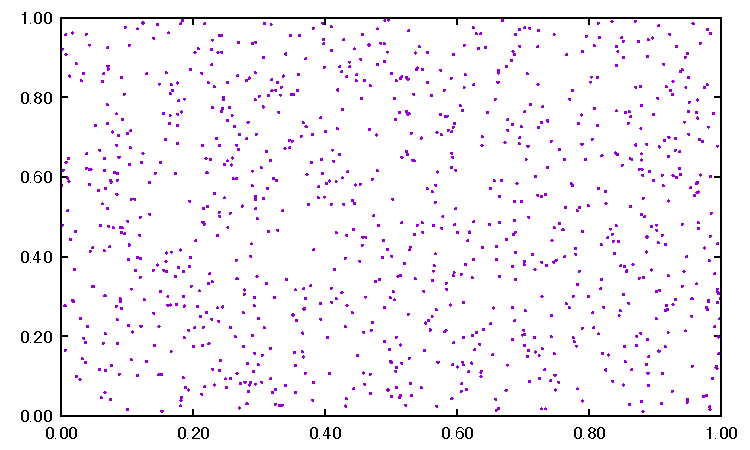
\includegraphics[width=.8\textwidth]{bsc-plot}
        \end{center}
        \caption{Many dots distributed over a two dimensional unit space
        without any discernible pattern or deeper meaning}
    \end{figure}


    \section{Evaluation of the results}

    Summarize the main aspects and results of the research
    project. Provide an answer to the research questions stated earlier.

    (target size: 1/2 page)


    \section{Conclusion}~\nocite{JS06}

    \newpage
    %\bibliographystyle{unsrt}
    %\bibliography{bsc-sample}
    \printbibliography

\end{document}